%!TEX program = xelatex
\documentclass{beamer}

\usepackage{blindtext}

\usepackage[T1]{fontenc}
\usepackage[font=small,labelfont=bf,tableposition=top]{caption}
\renewcommand{\figurename}{}
\usepackage{graphicx}



\usetheme{Execushares}

\title{Sistema Integrado de Consulta a Licitações Públicas}
\subtitle{Alex Sandro da Silva Magalhães Junior,\\ André Lucas Rodrigues da Silva}

\author{Instituto Federal de Goiás - Câmpus Formosa 2018}
\date{}
\setcounter{showSlideNumbers}{1}

\begin{document}
	\setcounter{showProgressBar}{0}
	\setcounter{showSlideNumbers}{0}

	\frame{\titlepage}

	\begin{frame}
		\frametitle{Agenda}
		\begin{enumerate}
			\item Processo Licitatório\\ %\textcolor{ExecusharesGrey}{\footnotesize\hspace{1em} Histórico}\\
			%\textcolor{ExecusharesGrey}{\footnotesize\hspace{1em} No Brasil}\\
			%\textcolor{ExecusharesGrey}{\footnotesize\hspace{1em} Definição}\\
			%\textcolor{ExecusharesGrey}{\footnotesize\hspace{1em} Processo Licitatório Contemporâneo}
			\textcolor{ExecusharesGrey}{\footnotesize\hspace{1em} Histórico, Definição e o Processo Contemporâneo}\\
			\item Fase Interna do Processo Licitatório\\
			\textcolor{ExecusharesGrey}{\footnotesize\hspace{1em} Como funciona}\\
			\item Análise e Desenvolvimento de Sistemas \\
			\textcolor{ExecusharesGrey}{\footnotesize\hspace{1em} Metodologia, ferramentas e tecnologias}\\
			 %\textcolor{ExecusharesGrey}{\footnotesize\hspace{1em} Visão Geral}\\
			%\begin{itemize}
				%\item Metodologias de desenvolvimento de software\\ 
				%\item Levantamento de requisitos\\ 
				%\item Implementação\\ %\textcolor{ExecusharesGrey}{\footnotesize\hspace{1em} Conceitos e Tecnologias}
				%\item Homologação e Implantação\\
				%\item Processo de software\\
			%\end{itemize}
			%%%%%%%%%%%%%%%%%%%%%%%%%%%%%%%%%%%%%%%%%%%%%%%%%%%%%%%%%%%%%%%%%%%%%%%%%%%%%%%%%%%%%%%%%
			\item Método\\
			\textcolor{ExecusharesGrey}{\footnotesize\hspace{1em} Aplicação}\\			 
			%\textcolor{ExecusharesGrey}{\footnotesize\hspace{1em} Processo de software}\\
			%\textcolor{ExecusharesGrey}{\footnotesize\hspace{1em} Levantamento de requisitos}\\
			%\textcolor{ExecusharesGrey}{\footnotesize\hspace{1em} Implementação do sistema}\\
			%\textcolor{ExecusharesGrey}{\footnotesize\hspace{1em} Implantação do sistema}
			\item Resultado\\ 
			%\textcolor{ExecusharesGrey}{\footnotesize\hspace{1em} Disponibilidade do sistema}
			\item Conclusão\\
		\end{enumerate}
	\end{frame}

	\setcounter{framenumber}{0}
	\setcounter{showProgressBar}{2}
	\setcounter{showSlideNumbers}{2}
	
	%%%%%%%%%%%%%%%%%%%%%%%%%%%%%%%%%%%%%%%%%%%%%%%%%%%%%%%%%%%%%%%%%%%%%%%%%%%%%%%%%%%%%%%%%
	\section{Processo Licitatório}
	
		\begin{frame}\frametitle{Histórico}
			\begin{itemize}
				\item Existe desde a Roma Antiga de VIII a.C.
				\item No Brasil
				\begin{itemize}
					\item Iniciou-se com o Decreto nº 2.962 de 1862
					\item Em âmbito federal, a partir do Decreto nº 4.536 de 1922
					\item Sistematização do tema com o Decreto-Lei nº 200 de 1962 no âmbito federal
					\item Estendida para as administrações dos estados e municípios pela Lei nº 545 de 1968
					\item Criou-se um Estatuto Jurídico das Licitações e Contratos Administrativos com os Decretos-Lei 2.348 e 2.360 de 1987
					\item Com a Constituição Federal de 1988, ganha \textit{status} de princípio constitucional
				\end{itemize}	
			\end{itemize}
		\end{frame}
	
		\begin{frame} \frametitle{Definição}
			\begin{itemize}
				\item Licitação vem do latim \textit{licitatione} 
				\item Significa venda por lances
				
			\end{itemize}
		\begin{block}{Definição}
			Procedimento administrativo da Administração Pública, que visa adquirir bens ou serviços,
			através da seleção da proposta mais benéfica, proporcionando igualdade nas condições dos que participem, buscando através do Contrato Administrativo
			impulsionar os ganhos da coletividade
		\end{block}
		\end{frame}	
	
		\begin{frame} \frametitle{Processo Licitatório Contemporâneo}
			\begin{itemize}
				\item Lei nº 8.666 de 1993 - normas gerais para licitações e contratos
				\item Artigos 22 e 23, da Lei nº 8.666 de 1993 prevêem cinco modalidades de licitação:
					\begin{itemize}
						\item Concorrência
						\item Tomada de preço
						\item Convite
						\item Concurso
						\item Leilão
					\end{itemize}
			\end{itemize}
		\end{frame}		
	
		\begin{frame}\frametitle{Processo Licitatório Contemporâneo}
			\begin{itemize}
				\item Medida Provisória nº 2.026 de 2000, cria a nova modalidade licitatória de Pregão
				\item Lei Federal nº 10.520 de 2002, estendeu a aplicação do Pregão modalidade também aos Estados e Municípios
				\item Melhoria do Pregão que é o Pregão eletrônico
				\item Regulamentada pelo Decreto nº 5.450 de 2005
			\end{itemize}
		\end{frame}
		
	%%%%%%%%%%%%%%%%%%%%%%%%%%%%%%%%%%%%%%%%%%%%%%%%%%%%%%%%%%%%%%%%%%%%%%%%%%%%%%%%%%%%%%%%%
	\section{Fase Interna do Processo Licitatório}
		\begin{frame}\frametitle{O Funcionamento}
			
			\begin{itemize}
				\item É um processo interno a um órgão da Administração Pública
				\item Advêm da necessidade de contratação ou aquisição de serviço ou de material
			
				\item O sucesso da fase interna depende de:
				\begin{itemize}
					\item eficiência
					\item economicidade
				\end{itemize}
			\end{itemize}
		\end{frame}
	
	\section{Problema}
	\begin{frame}\frametitle{Problema}
	
	Ausência de um meio eficiente de comunicação \textit{inter-campi} para alcançar o Princípio
	Constitucional da Eficiência na fase interna de processos licitatórios no IFG
	
	\end{frame}

	\section{Objetivo}
	\begin{frame}\frametitle{Objetivo}
	\begin{block}{Objetivo}
		Construir um sistema de comunicação \textit{inter-campi} para melhorar a fase interna de
		processos licitatórios no IFG
	\end{block}
	\begin{block}{Objetivos específicos}

	\begin{itemize}
		\item Criar um sistema, através do qual as partes interessadas poderão estabelecer rotinas
		legais e bem definidas abrangendo o máximo de demandas de compras em um único
		processo licitatório
		\item Apoiar as tomadas de decisão, a inteligência organizacional e a segurança da informação
		com vistas à redução de erros, custos e desperdícios, e ao aumento da
		precisão e produtividade
	\end{itemize}
	\end{block}	
	\end{frame}

	%%%%%%%%%%%%%%%%%%%%%%%%%%%%%%%%%%%%%%%%%%%%%%%%%%%%%%%%%%%%%%%%%%%%%%%%%%%%%%%%%%%%%%%%%
	\section{Análise e Desenvolvimento de Sistemas}
	
	\begin{frame}\frametitle{Visão Geral}
		Desenvolvimento de sistemas baseia-se essencialmente, em seguir etapas (ALVARENGA, 2016)
		
		\begin{itemize}
			\item Metodologias de desenvolvimento de software
			\begin{itemize}
				\item Metodologias tradicionais
				\item Metodologias ágeis
			\end{itemize}
			\item Levantamento de requisitos
			\begin{itemize}
				\item Com o uso de modelos abstratos e precisos, o levantamento de requisitos permite modelar um sistema
			\end{itemize}
			\item Implementação
			\begin{itemize}
				\item Fase posterior ao levantamento de requisitos
			\end{itemize}	
		\end{itemize}
	\end{frame}


	\begin{frame}\frametitle{Aplicação web}
		Uma aplicação web é qualquer software que é executado em um navegador (SAMPAIO, 2004)
		\begin{itemize}
			\item \textit{Back-end}
			\item \textit{Front-end}
		\end{itemize}
		\begin{figure}[ht]
			\centering
			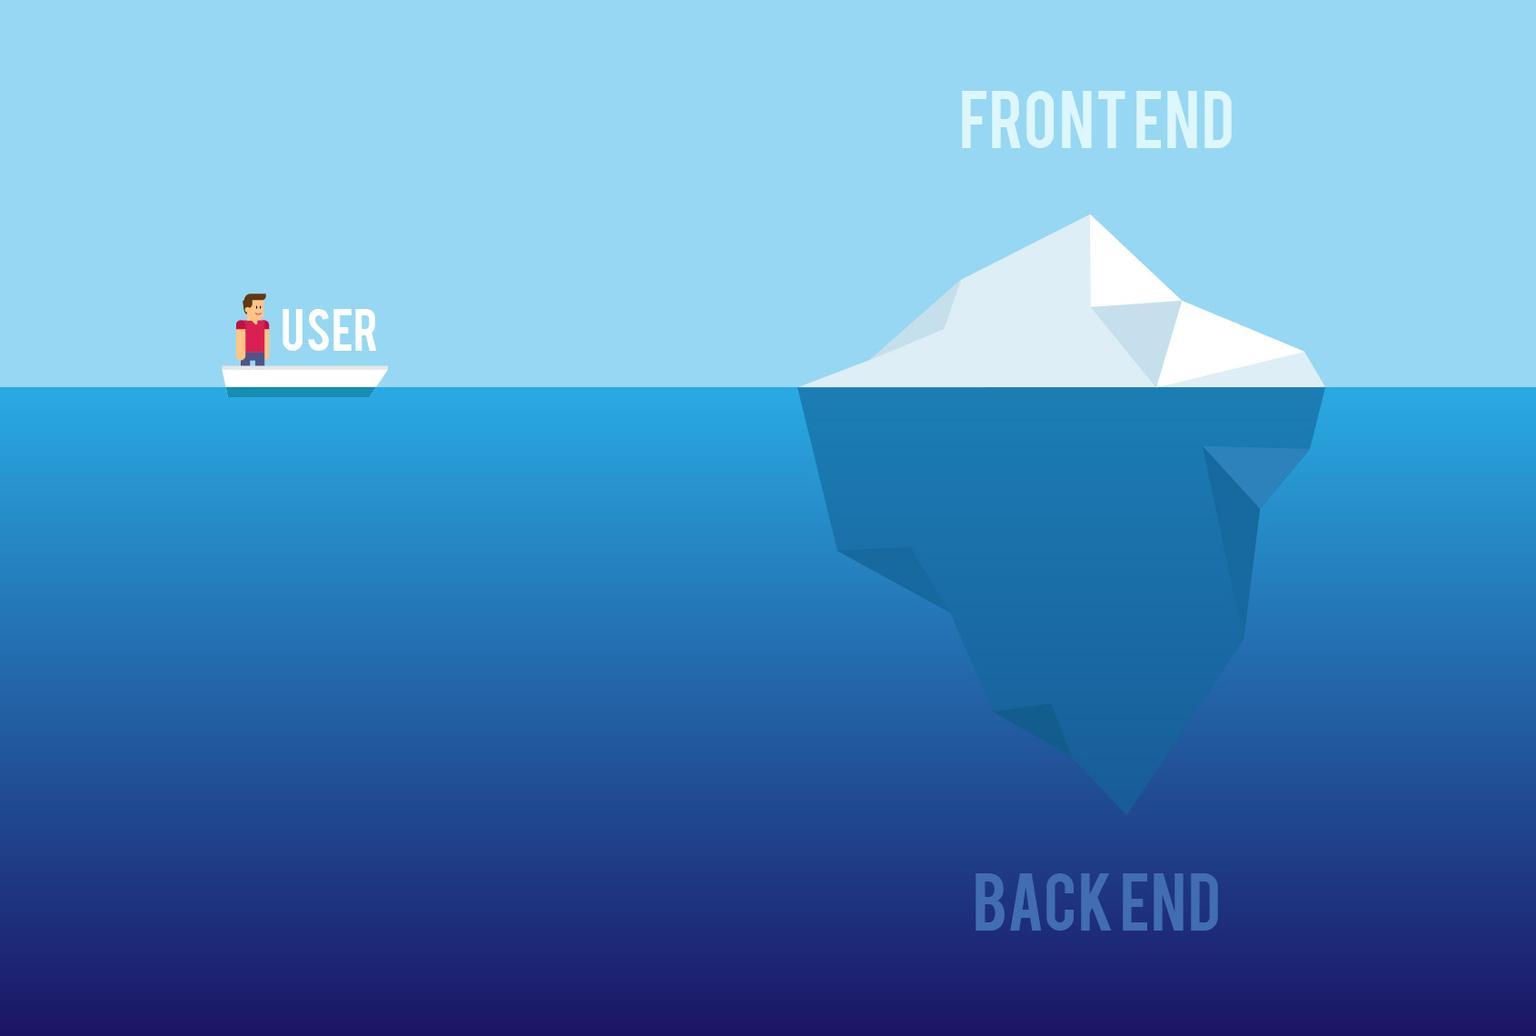
\includegraphics[scale=.11]{img/front-back.jpg}
		\end{figure}
	\end{frame}

	\begin{frame}\frametitle{Aplicação Web}
		\begin{itemize}
			\item Os \textit{Frameworws} são esqueletos de uma aplicação e possuem conjuntos já definidos e diversas estruturas prontas
			\item \textit{Representational State Transfer} (REST) é uma arquitetura baseado no protocolo \textit{HyperText Transfer Protocol} (HTTP) que serve para definir como é a comunicação entre sistemas de informação e a transferência de dados entre eles
		\end{itemize}
	\end{frame}


	\begin{frame}\frametitle{Ferramentas}
		\begin{itemize}
			\item As linguagens de programação são utilizadas como meio de comunicação entre computadores e desenvolvedores
			\item Um sistema de banco de dados é um sistema computadorizado de manutenção de registros cuja finalidade é armazenar informações e permitir que o usuário busque e atualize essas informações quando solicitado (DATE, 2004)
		\end{itemize}
	\end{frame}

	\begin{frame}\frametitle{Ferramentas}
		Application Programming Interface (API) é um conjunto estabelecido de mensagem que utilizam os métodos HTTP
			\begin{figure}[ht]
				\centering
				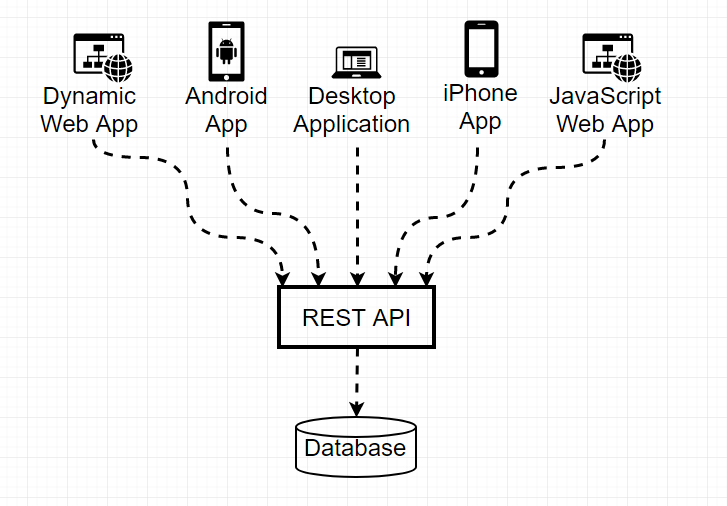
\includegraphics[scale=0.375]{img/rest_api.png}
			\end{figure}
	\end{frame}

	\begin{frame}\frametitle{Tecnologias}
		\begin{itemize}
			\item Java é uma linguagem de programação
			\item Spring boot é um \textit{framework} que acelera a programação de aplicações Java
			\item \textit{Hibernate} é um \textit{framework} para a comunicação entre a aplicação e o banco de dados através de \textit{Java Persistence API} (JPA)
			\item MySQL é um Sistema Gerenciador de Bancos de Dados (SGBD)
		\end{itemize}
	\end{frame}

	\begin{frame}\frametitle{Tecnologias}
		\begin{itemize}
			\item \textit{Hypertext Markup Language} (HTML) e \textit{Cascading Style Sheets} (CSS) servem para estruturar a apresentação e conteúdo

			\item JavaScript é uma linguagem de programação que fornece interatividade
			\item O \textit{Bootstrap} é um \textit{framework} que une HTML, CSS, e JavaScript.
			\item O AngularJS é um \textit{framework} JavaScript 
		\end{itemize}
	\end{frame}

	\begin{frame}\frametitle{Homologação e Implantação}
		\begin{itemize}
		\item A homologação é a fase onde o cliente e os interessados pelo produto, verificaram que o software feito atende aos critérios de aceite previamente estabelecidos com o cliente
		\item Após a aprovação do cliente o produto é entregue, e o cliente pode implantar o software em seu ambiente de produção
		\end{itemize}
	\end{frame}

	\begin{frame}\frametitle{Processo de software}
		Processo de software é um conjunto de atividades e resultados associados que produzem um produto de software (SOMMERVILLE, 2007)
		\begin{itemize}
			\item Especificação de software
			\item Design e implementação do software
			\item Verificação e validação
			\item Manutenção do software
		\end{itemize}
	\end{frame}

	\section{Método}
	
		\begin{frame}\frametitle{Processo de software}
			
			Utilizamos no processo de software o Scrum
		\end{frame}
	
		\begin{frame}\frametitle{Levantamento de requisitos}
			Através do levantamento de requisitos determinamos os problemas
			\begin{itemize}
				\item Problemas
				\begin{itemize}
					\item Descentralização das informações necessárias
					\item Problemas de comunicação entre os interessados
					\item Problemas de comunicação na fase interna
					\item Problema com a solicitação de pedidos
				\end{itemize}					
				\item Soluções propostas como caso de uso
				\begin{itemize}
					\item Inserção de dados
					\item Solicitar Inclusão
					\item Analisar Requisições
					\item Resposta Requisições
				\end{itemize}
			\end{itemize}
		\end{frame}
	
		\begin{frame}\frametitle{Implementação do sistema}
			A implementação da aplicação foi baseada em uma stack (pilha) de programas
			\begin{figure}[ht]
				\centering
				\includegraphics[scale=0.275]{img/arquitetura.png}
			\end{figure}
		\end{frame}
	
		\begin{frame}\frametitle{Implantação do sistema}
			A implantação do sistema ainda não ocorreu
		\end{frame}
	
	\section{Resultado}
		
		\begin{frame}\frametitle{Resultado}
			
			Os sistema está disponível no GitHub no endereço: <https://github.com/dragao1995/
			licitacaoweb> sob a Licença Apache 2.0
		\end{frame}

	\section{Conclusão}
	
		\begin{frame}\frametitle{Conclusão}
		
			A aplicação LicitaçãoWeb permite melhorar a comunicação na fase interna de um processo de licitação, colaborando com o princípio constitucional da eficiência
		\end{frame}	
	
	\section{Obrigado}
		
\end{document}
